%%%%%%%%%%%%%%%%%%%%%%%%%%%%%%%%%%%%%%%%%%%%%%%%%%%%%%%%%%%%%%%%
%%%%%%%%%%%%%%%%%%%%%%%%%%% Metadata %%%%%%%%%%%%%%%%%%%%%%%%%%%
%%%%%%%%%%%%%%%%%%%%%%%%%%%%%%%%%%%%%%%%%%%%%%%%%%%%%%%%%%%%%%%%
\documentclass{Axon}

\title{Discrete Mathematics and its Applications, 8th Edition - Chapter 1 The Foundations: Logic and Proofs - Section 1.2 Applications of Propositional Logic - Subsection 1.2.6 Logic Circuits}

\authors{
    \addauthor{Jeffrey G. Lind III}{jeffrey@jeffreylind.dev}
}

\addbibresource{Bibliography.bib}
%%%%%%%%%%%%%%%%%%%%%%%%%%%%%%%%%%%%%%%%%%%%%%%%%%%%%%%%%%%%%%%%
%%%%%%%%%%%%%%%%%%%%%%%%%%%%% Paper %%%%%%%%%%%%%%%%%%%%%%%%%%%%
%%%%%%%%%%%%%%%%%%%%%%%%%%%%%%%%%%%%%%%%%%%%%%%%%%%%%%%%%%%%%%%%
\begin{document}
\maketitle
\makeauthor
%%%%%%%%%%%%%%%%%%%%%%%%%%%%%%%%%%%%%%%%%%%%%%%%%%%%%%%%%%%%%%%%
%%%%%%%%%%%%%%%%%%%%%%%%%%% Abstract %%%%%%%%%%%%%%%%%%%%%%%%%%%
%%%%%%%%%%%%%%%%%%%%%%%%%%%%%%%%%%%%%%%%%%%%%%%%%%%%%%%%%%%%%%%%
\begin{abstract}
Notes on Discrete Mathematics and its Applications, 8th Edition - Chapter 1 The Foundations: Logic and Proofs - Section 1.2 Applications of Propositional Logic - Subsection 1.2.6 Logic Circuits \cite{Rosen}.
\end{abstract}
%%%%%%%%%%%%%%%%%%%%%%%%%%%%%%%%%%%%%%%%%%%%%%%%%%%%%%%%%%%%%%%%
%%%%%%%%%%%%%%%%%%%%%%%%%%% Section 1 %%%%%%%%%%%%%%%%%%%%%%%%%%
%%%%%%%%%%%%%%%%%%%%%%%%%%%%%%%%%%%%%%%%%%%%%%%%%%%%%%%%%%%%%%%%
\section{Introduction}
Propositional logic can be applied to the design of computer hardware. This was first observed in 1938 by Claude Shannon in his MIT master's thesis. In Chapter 12 we will study this topic in depth. (See that chapter fro a biography of Shannon.) We give a brief introduction to this application here.

A \textbf{logic circuit} (or \textbf{digital circuit}) receives input signals \(p_1, p_2, \ldots, p_n\), each a bit [either \(0\) (off) or \(1\) (on)], and produces output signals \(s_1, s_2, \ldots, s_n\), each a bit. In this section we will restrict our attention to logic circuits with a single output signal; in general, digital circuits may have multiple outputs.

Complicated digital circuits can be constructed from three basic circuits, called \textbf{gates}, shown in Figure \ref{Figure: 1}. The \textbf{inverter}, or \textbf{NOT gate}, takes an input bit \(p\), and produces as output \(\lnot p\). The \textbf{OR gate} takes two input signals \(p\) and \(q\), each a bit, and produces as output the signal \(p \lor q\). Finally, the \textbf{AND gate} takes two input signals \(p\) and \(q\), each a bit, and produces as output the signal \(p \land q\). We use combinations of these three basic gates to build more complicated circuits, such as that shown in Figure \ref{Figure: 2}

\begin{figure}[h]
    \centering
    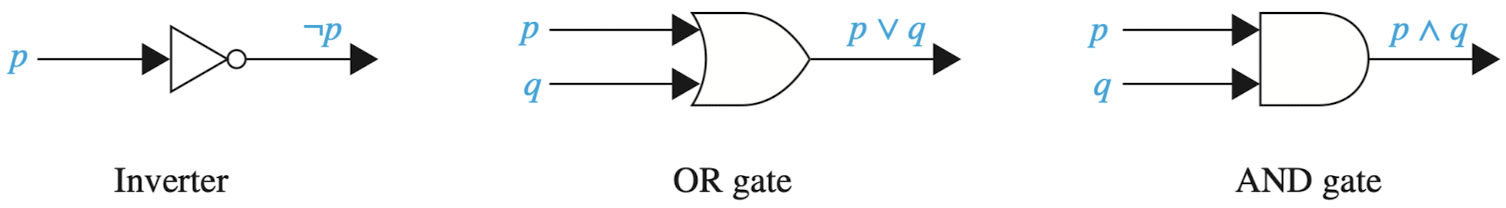
\includegraphics[width=0.75\linewidth]{Discrete Mathematics and its Applications, 8th Edition/Chapter 1 Logic and Proofs/Section 1.2 Applications of Propositional Logic/Figure 1.png}
    \caption{Basic logic gates.}
    \label{Figure: 1}
\end{figure}

Given a circuit built from the basic logic gates and the inputs to the circuit, we determine the output by tracing through the circuit, as Example \ref{Example: 10} shows.

\begin{example}\label{Example: 10}
    Determine the output for the combinatorial circuit in Figure \ref{Figure: 2}

    \noindent
    \textbf{Solution:}
    In Figure \ref{Figure: 2} we display the output of each logic gate in the circuit. We see that the AND gate takes input of \(p\) and \(\lnot q\), the output of the inverter with input \(q\), and produces \(p \land \lnot q\). Next, we note that the OR gate takes inputs \(p \land \lnot q\) and \(\lnot r\), the output of the inverter with input \(r\), and produces the final output \((p \land \lnot q) \lor \lnot r\).
\end{example}

Suppose that we have a formula for the output of a digital circuit in terms of negations, disjunctions, and conjunctions. Then, we can systematically build a digital circuit with the desired output, as illustrated in Example \ref{Example: 11}.
\begin{figure}[h]
    \centering
    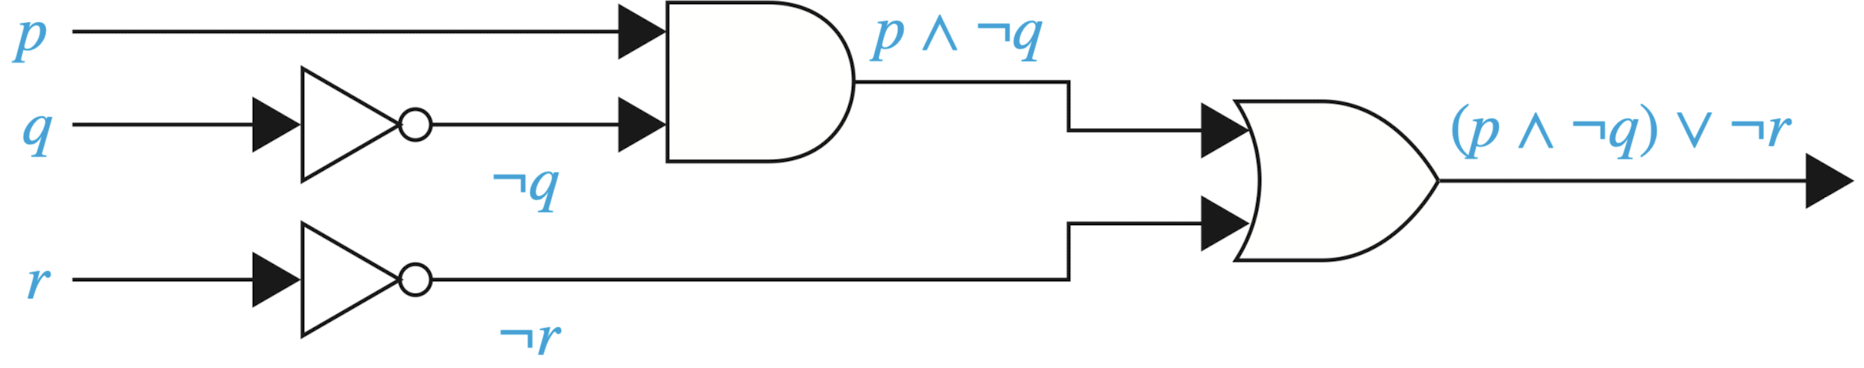
\includegraphics[width=0.75\linewidth]{Discrete Mathematics and its Applications, 8th Edition/Chapter 1 Logic and Proofs/Section 1.2 Applications of Propositional Logic/Figure 2.png}
    \caption{A combinatorial circuit}
    \label{Figure: 2}
\end{figure}

\begin{figure}[ht]
    \centering
    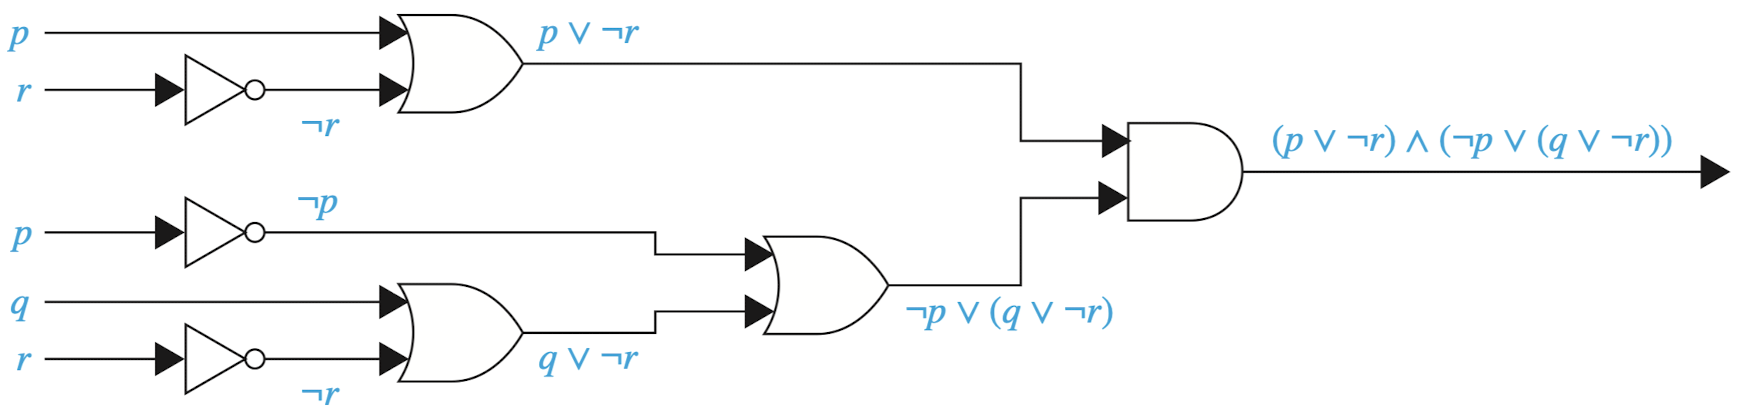
\includegraphics[width=0.75\linewidth]{Discrete Mathematics and its Applications, 8th Edition/Chapter 1 Logic and Proofs/Section 1.2 Applications of Propositional Logic/Figure 3.png}
    \caption{The circuit for \((p \lor \lnot r) \land (\lnot p \lor (q \lor \lnot r))\)}.
    \label{Figure: 3}
\end{figure}

\begin{example}\label{Example: 11}
    Build a digital circuit that produces the output \((p \lor \lnot r) \land (\lnot p \lor (q \lor \lnot r))\) when given input bits \(p\), \(q\), and \(r\).

    \noindent
    \textbf{Solution:}
    To construct the desired circuit, we build separate circuits for \(p \lor \lnot r\) and for \(\lnot p \lor (q \lor \lnot r)\) and combine them using an AND gate. To construct a circuit for \(p \lor \lnot r\), we use an inverter to produce \(\lnot r\) from the input \(r\). Then, we use an OR gate to combine \(p\) and \(\lnot r\). To build a circuit for \(\lnot p \lor (q \lor \lnot r)\), we first use an inverter to obtain \(\lnot r\). Then we use an OR gate with inputs \(q\) and \(\lnot r\) to obtain \(q \lor \lnot r\). Finally, wee use another inverter and an OR gate to get \(\lnot p \lor (q \lor \lnot r)\) from the inputs \(p\) and \(q \lor \lnot r\).

    To complete the construction, we employ a final AND gate, with inputs \(p \lor \lnot r\) and \(\lnot p \lor (q \lor \lnot r)\). The resulting circuit is displayed in Figure \ref{Figure: 3}.
\end{example}

We will study logic circuits in great detail in Chapter 12 in the context of Boolean algebra, and with different notation.

\printbibliography

\end{document}